\documentclass{article}
\usepackage{graphicx}

\title{Advanced Machine Learning Assignment 3}
\author{Divij Singh}
\date{20/02/19}


\begin{document}

	\maketitle
	
	\section{Q1}
(a)\\
Yes, A is independant of B in both cases 2 and 3, as neither B nor D occuring influence the occurence of A.\\\\
(b) \\
In case 2, B is conditionally independant of D given A, but not given C. In case 3, B is conditionally independant of D given either A or C.

\section{Q2}
For this question, since Heart Disease is only dependant on Exercise and Healthy Diet, we can ignore blood pressure.\\
$P(HD,E,D)= P(HD|E,D)P(E)P(D) = (0.25 x 0.7 x 0.25) = 0.04375$\\
Thus we have the probability of the individual having heart disease.

\section{Q3}
For this problem, we take some assumed values of Sysadmin Upgrade, Attempted Intrusion, A1, A2, and Detection of Intrusion as outlined in the graph.\\
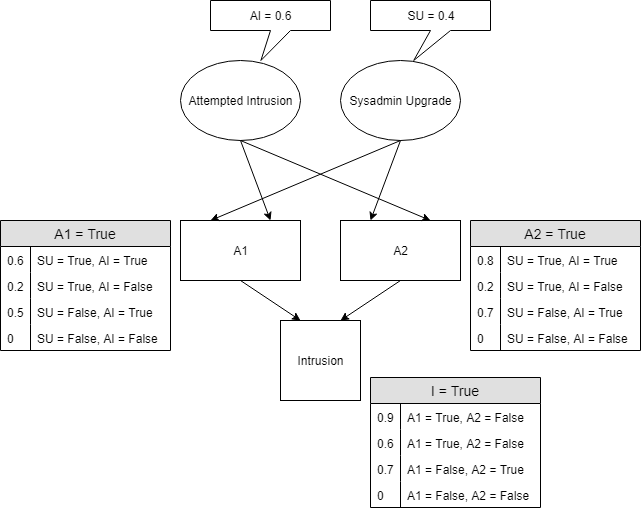
\includegraphics[scale = 0.5]{Q3 Diagram.png}\\
$Pr(SU,AI,A1) = Pr(A1|SU,AI)Pr(SU)Pr(AI)$\\
We take the sum of each possibility.\\
$(0.6 * 0.6 * 0.4) + (0.2 * 0.4 * 0.6) + (0.5 * 0.4 * 0.6) + (0) = 0.312$\\\\

$Pr(\neg A2,SU,AI) = Pr(\neg A2|SU,AI)Pr(SU)Pr(AI)$\\
We take the sum of each possibility.\\
$(0.2 * 0.6 * 0.4) + (0.8 * 0.4 * 0.6) + (0.3 * 0.4 * 0.6) + (0) = 0.312$\\\\

$Pr(I,A1,A2) = Pr(I|A1,A2)Pr(A1)Pr(A2)$\\
We take the sum of each possibility.\\
$(0.9 * 0.312 * 0.688) + (0.6 * 0.312 * 0.312) + (0.7 * 0.688 * 0.312) + (0) = 0.0378$\\
Thus it is unlikely to be an intrusion.
\end{document}